\documentclass[14pt,a1paper,landscape]{tikzposter}

%% Tikzposter is highly customizable: please see
%% https://bitbucket.org/surmann/tikzposter/downloads/styleguide.pdf

%% Available themes: see also
%% https://bitbucket.org/surmann/tikzposter/downloads/themes.pdf
% \usetheme{Default}
% \usetheme{Rays}
% \usetheme{Basic}
% \usetheme{Simple}
 \usetheme{Envelope}
% \usetheme{Wave}
% \usetheme{Board}
% \usetheme{Autumn}
% \usetheme{Desert}

%% Further changes to the title etc is possible
% \usetitlestyle{Default}
% \usetitlestyle{Basic}
 \usetitlestyle{Empty}
% \usetitlestyle{Filled}
% \usetitlestyle{Envelope}
% \usetitlestyle{Wave}
% \usetitlestyle{verticalShading}


%\usepackage{fontspec}
%\setmainfont{FreeSerif}
%\setsansfont{FreeSans}
\usetikzlibrary{positioning}
\usepackage{listings}
\usepackage{color}
%\usetikzlibrary{trees}
\usepackage[edges]{forest}
\usepackage [sfdefault]{cabin}
\usepackage[T1]{fontenc}
\usepackage{natbib}
\usepackage{wrapfig}
\definecolor{mymauve}{rgb}{0.58,0,0.82}

\author{Eric Rexstad, David L. Miller, Laura Marshall and Len Thomas}
\title{\parbox{0.6\linewidth}{\centering Migrating distance sampling projects from Distance for Windows to the Distance R package}}
\institute{Centre for Research into Ecological and Environmental Modelling University of St Andrews}


% borrowed from https://tex.stackexchange.com/questions/185166/tikzposter-4-logos-title-2-at-each-side/185278#185278

%\makeatletter
%\def\TP@titlegraphictotitledistance{-4cm}
%\settitle{ \centering \vbox{
%		\@titlegraphic \\ [\TP@titlegraphictotitledistance] 
%		\centering
%		\color{titlefgcolor} {\bfseries \Huge \sc \@title \par}
%		\vspace*{1em}
%		{\huge \@author \par} \vspace*{1em} {\LARGE \@institute}
%}}
%\makeatother

%\setlength{\columnsep}{2cm}
%
%\title{\parbox{0.5\linewidth}{\centering My  really  really  really  really  really  really  really  really  long poster TITLE.}}
%\author{Name}
%\titlegraphic{
%	\includegraphics[width=8cm, height=4cm]{ISEC_Logo.png}
%	\hfill 
%%	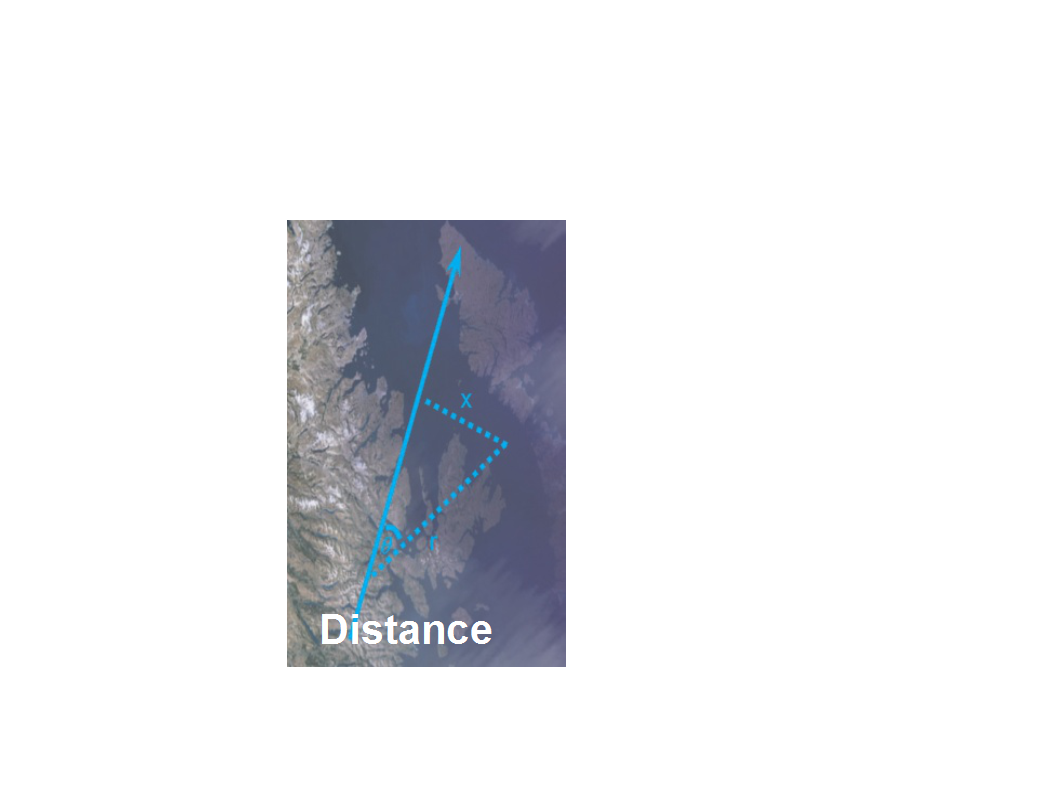
\includegraphics[width=9cm,height=8cm]{distancelogo.png}
%	\\% \vspace{5pt} \\
%	
\includegraphics[width=3cm, height=6cm]{02-foundation-vertical-white.png}
%	\hfill 
%	\includegraphics[width=10.5cm,height=3cm]{CREEM_Logo_trans.png}
%}


%% Original, functional way to place single logo in middle
%\titlegraphic{\includegraphics[width=7cm]{ISEC_Logo.png}}
%% Uncomment to switch off tikzposter footer
\tikzposterlatexaffectionproofoff

%%%%%%%%%%%%%%%  Yet another multi-logo title solution from THIS WORKS after adding \usetikzlibrary{positioning}
% https://tex.stackexchange.com/questions/263563/add-logos-beyond-the-title-tikzposter

\makeatletter
\newcommand\insertlogoi[2][]{\def\@insertlogoi{\includegraphics[#1]{#2}}}
\newcommand\insertlogoii[2][]{\def\@insertlogoii{\includegraphics[#1]{#2}}}
\newcommand\insertlogoiii[2][]{\def\@insertlogoiii{\includegraphics[#1]{#2}}}
\newcommand\insertlogoiv[2][]{\def\@insertlogoiv{\includegraphics[#1]{#2}}}
\newlength\LogoHSep
\newlength\LogoVSep

\setlength\LogoHSep{60pt}
\setlength\LogoVSep{1cm}

\insertlogoi[width=7cm]{ISEC_Logo_light_background_RGB.png}
\insertlogoii[width=7cm]{CREEM_Logo_trans.png}
\insertlogoiii[width=6cm]{02-foundation-vertical-white.png}
\insertlogoiv[width=12cm]{distancelogo.png}

\renewcommand\maketitle[1][]{  % #1 keys
	\normalsize
	\setkeys{title}{#1}
	% Title dummy to get title height
	\node[transparent,inner sep=\TP@titleinnersep, line width=\TP@titlelinewidth, anchor=north, minimum width=\TP@visibletextwidth-2\TP@titleinnersep]
	(TP@title) at ($(0, 0.5\textheight-\TP@titletotopverticalspace)$) {\parbox{\TP@titlewidth-2\TP@titleinnersep}{\TP@maketitle}};
	\draw let \p1 = ($(TP@title.north)-(TP@title.south)$) in node {
		\setlength{\TP@titleheight}{\y1}
		\setlength{\titleheight}{\y1}
		\global\TP@titleheight=\TP@titleheight
		\global\titleheight=\titleheight
	};
	
	% Compute title position
	\setlength{\titleposleft}{-0.5\titlewidth}
	\setlength{\titleposright}{\titleposleft+\titlewidth}
	\setlength{\titlepostop}{0.5\textheight-\TP@titletotopverticalspace}
	\setlength{\titleposbottom}{\titlepostop-\titleheight}
	
	% Title style (background)
	\TP@titlestyle
	
	% Title node
	\node[inner sep=\TP@titleinnersep, line width=\TP@titlelinewidth, anchor=north, minimum width=\TP@visibletextwidth-2\TP@titleinnersep]
	at (0,0.5\textheight-\TP@titletotopverticalspace)
	(title)
	{\parbox{\TP@titlewidth-2\TP@titleinnersep}{\TP@maketitle}};
	
	\node[inner sep=0pt,anchor=west]
	at ([shift={(-\LogoHSep,\LogoVSep)}]title.west)
	(logo1)
	{\@insertlogoi};
	
	\node[inner sep=0pt,anchor=west,right=of logo1] 
	(logo2)
	{\@insertlogoii};
	
	\node[inner sep=0pt,anchor=east] 
	at ([shift={(\LogoHSep,\LogoVSep)}]title.east)
	(logo4)
	{\@insertlogoiv};
	
	\node[inner sep=0pt,left=of logo4] 
	(logo4)
	{\@insertlogoiii};
	
	% Settings for blocks
	\normalsize
	\setlength{\TP@blocktop}{\titleposbottom-\TP@titletoblockverticalspace}
}
\makeatother

%%%%%%%%%%%%%%%%%%%%%%%%%%%%%%%%%%%%%%%%%%

\begin{document}
\maketitle

\begin{columns}

\column{0.333}

\block{Introduction}{
The Distance software \citep{thomas_distance_2010} has been downloaded >40,000 times in its 20-year history.  Much of the underlying machinery is written in R.  For some users, there may be benefits to performing the analysis with the underlying R code, rather than working with the graphical user interface (GUI).
	\begin{tikzfigure}[Traditional Distance for Windows interface (left) and distance sampling analysis in R (right).]
%		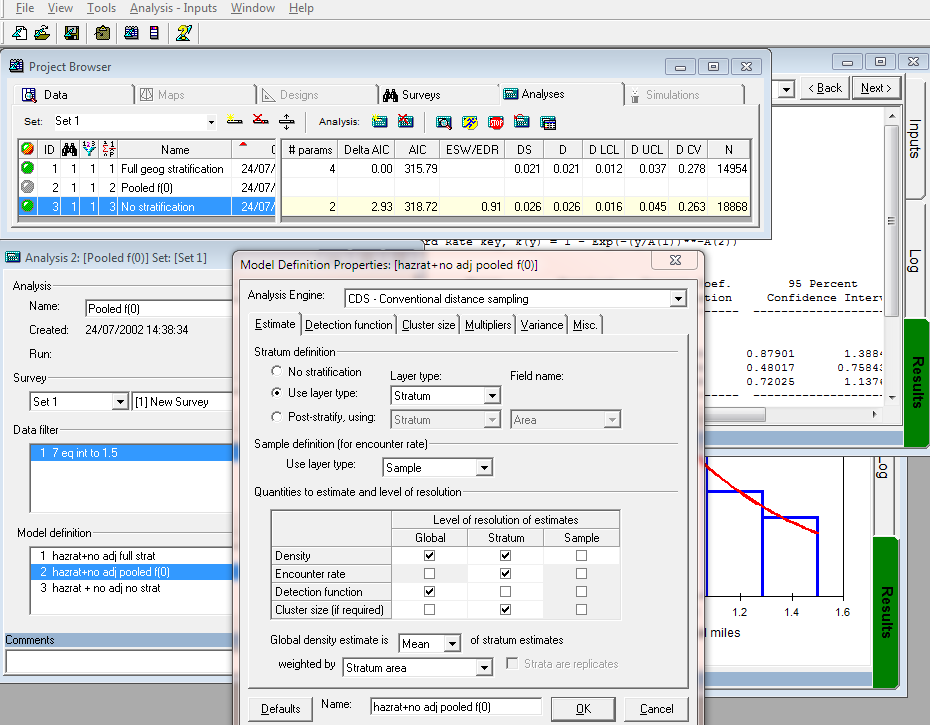
\includegraphics[width=0.45\columnwidth]{D7-analysis-grab.PNG}
		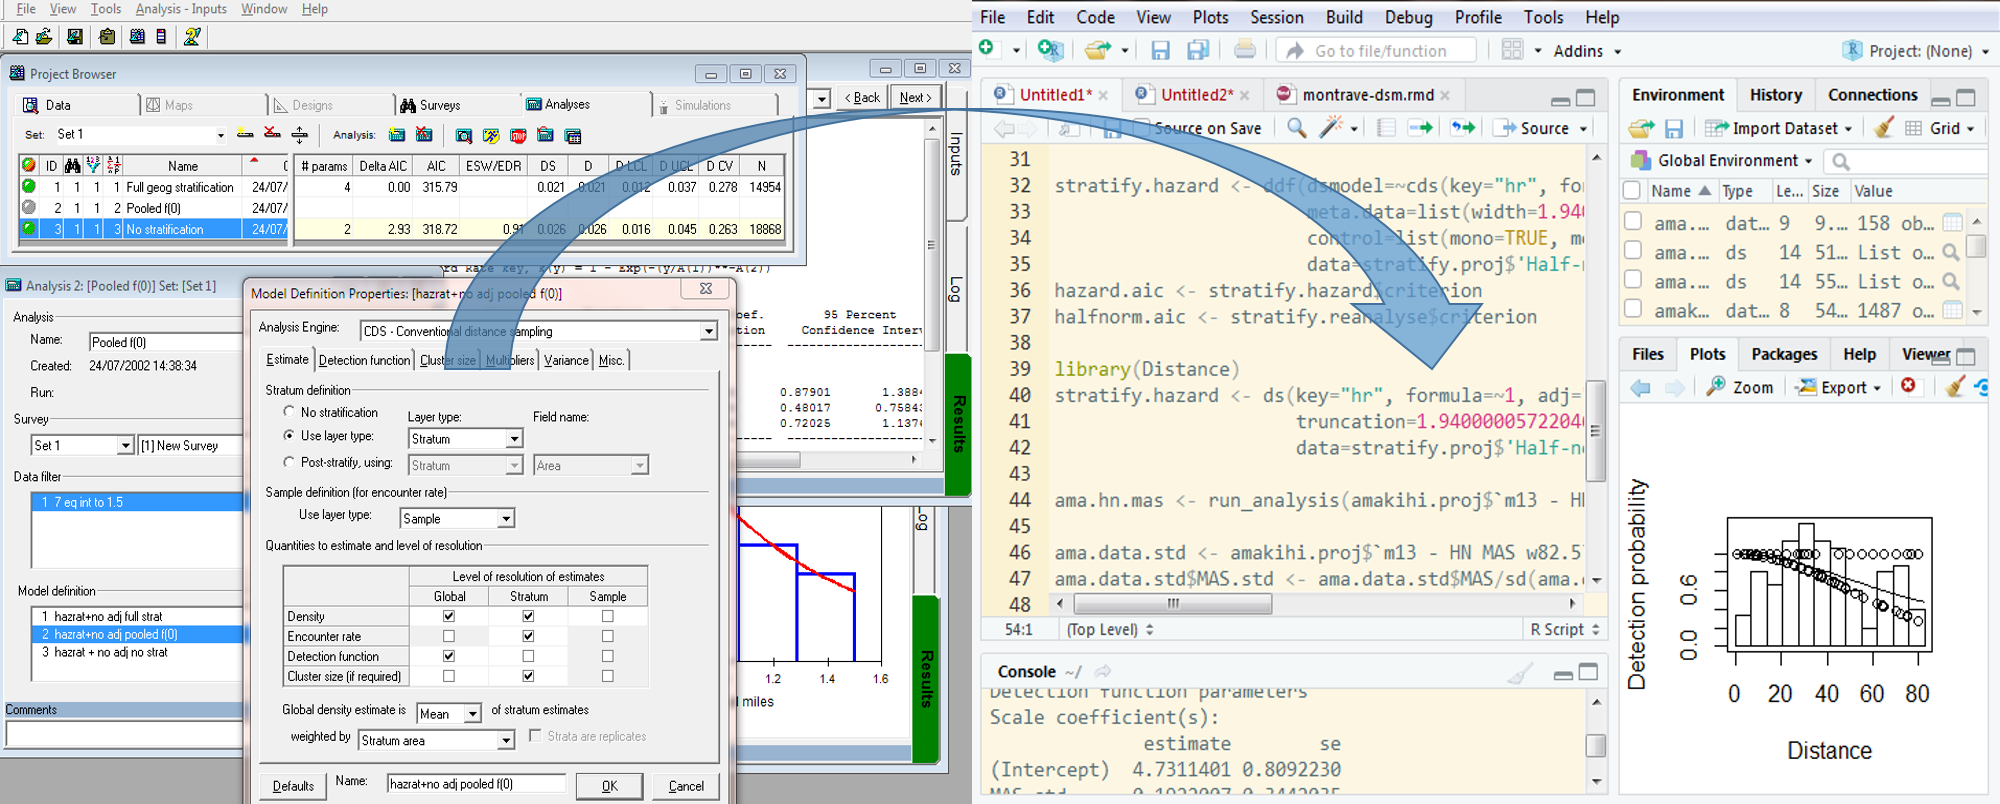
\includegraphics[width=0.95\linewidth]{merged-grabs.png}
%		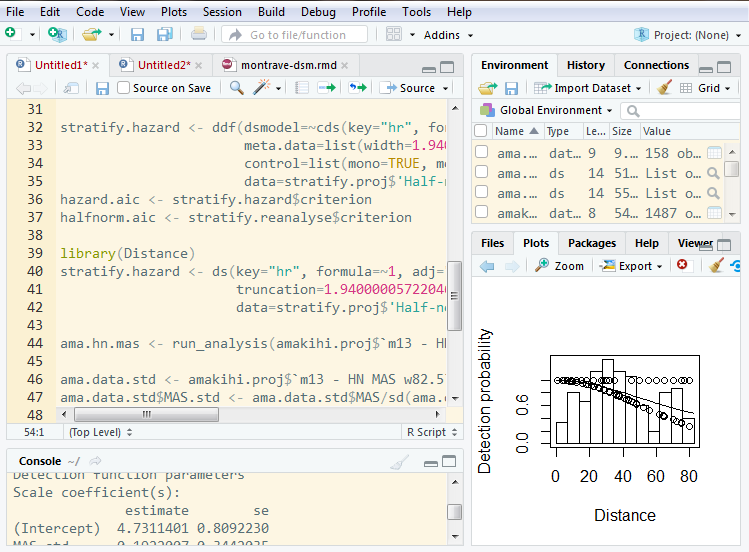
\includegraphics[width=0.45\columnwidth]{R-analysis-grab.PNG}
	\end{tikzfigure}

Challenges hindering the transition between analysis with the GUI and analyses in R are two-fold:
\begin{itemize}
	\item Legacy data reside in Distance (GUI) projects, unavailable for importing into R, and
	\item Analyses that are easily described using the GUI may be difficult to specify, particularly if analyst is not proficient in R.
\end{itemize}
}

\note[rotate=8, connection, width = 7cm, % targetoffsety=-2cm,
% roundedcorners=15, targetoffsetx=2cm
]{How to make this transition?}

\block{How to bridge between the two?}{

Distance GUI projects contain essential information necessary to conduct an analysis.  The fundamental purpose of the \texttt{readdst} package is to access this information and place it into R objects for further scrutiny.
 


\begin{wrapfigure}[12]{l}{0.6\linewidth}
	\begin{tikzfigure}
		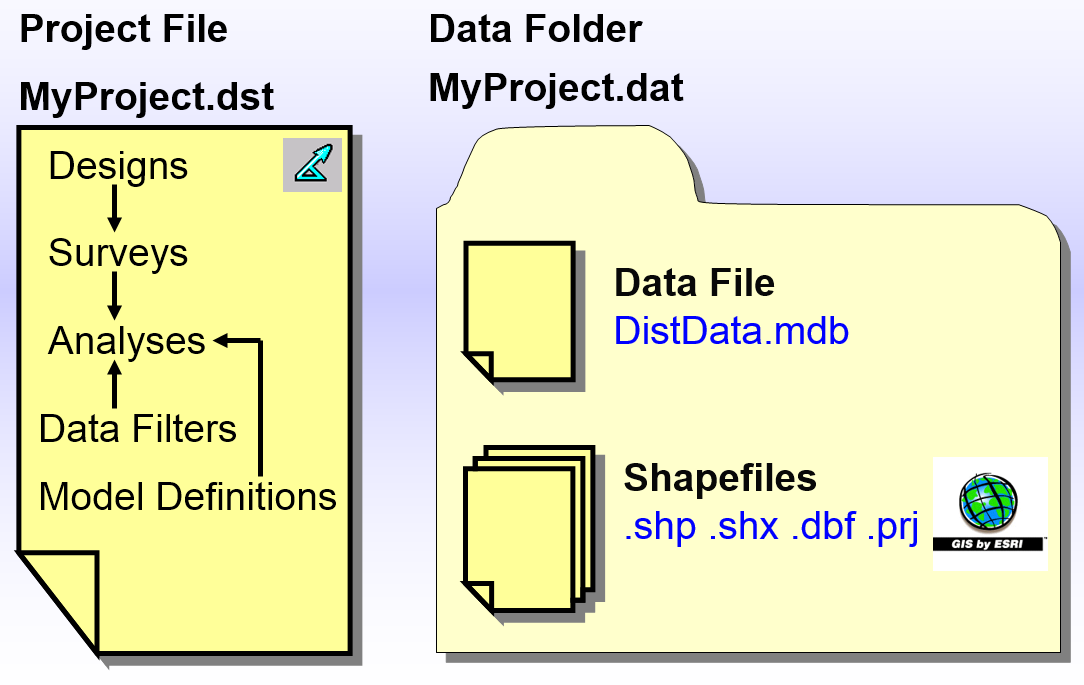
\includegraphics[width=.85\linewidth]{dst-file-structure.PNG}
	\end{tikzfigure}
	\caption{Database structure of a Distance project.}
\end{wrapfigure}

The elements of a distance sampling analysis are contained inside Distance project files in the form of an Access database.

\begin{enumerate}
	\item Data
	\item model definitions
	\item analysis results
\end{enumerate}

Mining information from tables within the database, via either \texttt{RODBC} (Windows) or \texttt{mdb-tools} (Macs).  Then it is a matter of performing the following three steps.

\begin{itemize}
	\item Trick is to extract contents of (2) and translate into R code
	\item Target the results of previous step to contents of (1) the data
	\item Perhaps contrast results of R analysis with results stored in the Access database
\end{itemize}

}

\column{0.3333}
\block{Applications--Legacy projects}
{
	Workhorse function in \texttt{readdst} package is \texttt{convert\_projects()}.  Its single argument is simply the complete location path to an existing Distance GUI project (created by either Distance 6 or 7).  \texttt{convert\_projects()} interrogates the Access database and translates the contents of data base tables into an R object of class \texttt{converted\_distance\_analyses}, a list of lists of class \texttt{converted\_distance\_analysis}.  Fig. \ref{fig:object} gives an outline of the content of this list.
}

	
%\usetikzlibrary{arrows,shapes,positioning,shadows,trees}
%
%\tikzset{
%	font={\fontsize{8pt}{8}\selectfont},		
%	basic/.style  = {draw, text width=2cm, drop shadow, rectangle},
%	root/.style   = {basic, rounded corners=2pt, thin, align=center,
%		fill=green!30},
%	level 2/.style = {basic, rounded corners=6pt, thin,align=center, fill=green!60,
%		text width=8em},
%	level 3/.style = {basic, thin, align=left, fill=pink!60, text width=6.5em}
%	level 4/.style = {basic, thin, align=left, fill=blue!60, text width=6.5em}
%}
%
%\begin{tikzfigure}[Structure of object produced by \texttt{convert\_project()}.]
%	\centering
%\begin{tikzpicture}[
%level 1/.style={sibling distance=40mm},
%edge from parent/.style={->,draw},
%>=latex]
%
%% root of the the initial tree, level 1
%\node[root] {converted\_distance\_analyses object}
%% The first level, as children of the initial tree
%child {node[level 2] (c1) {Half-normal cosine adjustments}}
%child {node[level 2] (c2) {Hazard rate Hermite adjustments}}
%child {node[level 2] (c3) {Uniform cosine adjustments}};
%
%% The second level, relatively positioned nodes
%\begin{scope}[every node/.style={level 3}]
%\node [below of = c1, xshift=15pt] (c11) {call mrds::ddf(dsmodel=$\sim$cds(key="hn", formula=$\sim$1, adj.series="cos"),...};
%\node [below of = c11] (c12) {filter=none};
%\node [below of = c12] (c13) {status=1};
%\node [below of = c13] (c14) {group size};
%\end{scope}
%child {node[level 4] (d1) {under here}}
%
%%\node [below of = c2, xshift=15pt] (c21) {Using a Matrix};
%%\node [below of = c21] (c22) {Relatively};
%%\node [below of = c22] (c23) {Absolutely};
%%\node [below of = c23] (c24) {Using overlays};
%%
%%\node [below of = c3, xshift=15pt] (c31) {Default arrows};
%%\node [below of = c31] (c32) {Arrow library};
%%\node [below of = c32] (c33) {Resizing tips};
%%\node [below of = c33] (c34) {Shortening};
%%\node [below of = c34] (c35) {Bending};
%%\end{scope}
%
%% lines from each level 1 node to every one of its "children"
%\foreach \value in {1,2,3}
%\draw[->] (c1.195) |- (c1\value.west);
%
%%\foreach \value in {1,...,4}
%%\draw[->] (c2.195) |- (c2\value.west);
%%
%%\foreach \value in {1,...,5}
%%\draw[->] (c3.195) |- (c3\value.west);
%\end{tikzpicture}
%\end{tikzfigure}



% filesystem tree from http://texample.net/tikz/examples/feature/trees/

%\begin{tikzfigure}[Structure of object produced by \texttt{convert\_project()}.]
%	\centering
%\tikzset{
%	font={\fontsize{8pt}{8}\selectfont}}	
%\tikzstyle{every node}=[draw=black,thick,anchor=west]
%\tikzstyle{selected}=[draw=red,fill=red!30]
%\tikzstyle{optional}=[dashed,fill=gray!50]
%\begin{tikzpicture}[%
%grow via three points={one child at (0.5,-0.7) and
%	two children at (0.5,-0.7) and (0.5,-1.4)},
%edge from parent path={(\tikzparentnode.south) |- (\tikzchildnode.west)}]
%\node {analysis\_object}
%child { node {call}}		
%child { node {aic.select}}
%child { node {status}}
%child { node [selected] {env}
%	child { node {data}}
%	child { node {obs.table}}
%	child { node {region.table}}
%	child { node {sample.table}}
%	child { node {units}}
%}
%child { node {filter}}
%child { node {group size}}
%	child { node {Bias}}
%	child { node {by}}
%child { node {detection\_by}}
%child { node {gof\_intervals}}
%child { node {estimation}}
%	child { node {by}}
%	child { node {Design}}
%	child { node {Weight}}
%child { node {ID}}
%child { node {engine}}
%child { node {project}}
%child { node {project\_file}};
%\end{tikzpicture}
%\end{tikzfigure}


\begin{subcolumns} 
	\subcolumn{.25}  
	
\block{}
{
	
% https://tex.stackexchange.com/questions/23647/drawing-a-directory-listing-a-la-the-tree-command-in-tikz	
\begin{tikzfigure}[Structure of object produced by \texttt{convert\_project()}.]
	\label{fig:object}
\begin{forest}
	for tree={%
		font=\footnotesize,
		folder,
		grow'=0,
		fit=tight,
	}
	[analysis\_object
	[call
	]
	[aic.select
	]
	[status
	]
	[env%,  label=right:where data reside
	[data]
	[obs.table]
	[region.table]
	[sample.table]
	[units]
	]
	[filter]
	[group\_size
%	[Bias]
%	[by]
	]
	[detection\_by]
	[gof\_intervals]
	[estimation
%	[by]
%	[Design]
%	[Weight]
	]
	[ID]
	[engine]
	[project]
	[project\_file]
	]
\end{forest}
\end{tikzfigure}
}

\subcolumn{.75} 

\block{Object produced by \texttt{convert\_project()}}
{
	
	Figure \ref{fig:object} (left) shows the structure of an object of type \texttt{converted\_distance\_analysis}.  There are as many of these produced by \texttt{convert\_project()} as there were analyses in the Distance project.
	
	The list contains all the salient information of a Distance analysis extracted from the Access database.  We point out several of the list elements critical to subsequent processing of the now-extracted data.
	\begin{description}
		\item [call] R code call to the function \texttt{mrds()} to duplicate the analyses done in the Distance GUI.
		\item [env] An \textit{environment} consisting of a set of data frames.  These data frames include the original data extracted from the Distance project, along with the observation, sample and region tables describing the hierarchial nature of the data base.
	\end{description}

	The nature of the analysis conducted by the Distance GUI, translated into a call to \texttt{mrds()} \citep{Laake2018}, as well as the data used in the analysis is contained within this object and available for further analysis within the R environment.
	
	The \texttt{converted\_distance\_analysis} list can be passed as an argument to \texttt{run\_analysis()}.  This function will perform an \texttt{mrds()} analysis \emph{behind-the-scenes} , without the user seeing how it was performed.
%	A standard use of the package is to convert and dataset and set of analyses from a Distance GUI project and re-run the analyses in R.  This is done using the workflow at left, based around the use of the \texttt{convert\_project()} function in concert with \texttt{run\_analysis()}
} 


\block{Learning structure of R interface}
{
	A user familiar with performing distance sampling analyses in the Distance GUI can use \texttt{converted\_distance\_analysis} objects to learn how to perform corresponding analyses using \texttt{mrds()}.  Alternatively, the imported data can be analysed using the Distance \citep{Miller2018} package.  Examples of both approaches provided below
%%%  fix to code inside block error -- https://tex.stackexchange.com/questions/228675/how-can-i-put-a-code-listing-in-a-tikzposter-block
	
	\lstset{language=R, backgroundcolor=\color{blue!10}, keywordstyle=\color{blue}, stringstyle=\color{mymauve}, basicstyle=\footnotesize}
    \lstinputlisting[fontadjust]{convert-stratify.r}
}

\end{subcolumns}

\column{0.3333}
\block{Comparative analysis of difficult data}{
	\begin{itemize}
		\item We try to do this. what?
		\item we try to do that.
	\end{itemize}
}

\block{Caveats}{
	\texttt{readdst} is not able to translate all GUI analyses into R code.  Current limitations are inability to translate
	\begin{itemize}
		\item analyses using the \texttt{dsm}, \texttt{mads} and \texttt{Dssim} engines,
		\item analyses using post-stratification and
		\item bootstraps for variance estimation.
	\end{itemize}
}

\block{Additional information}{

\coloredbox[]{
\nocite{*} % Insert publications even if they are not cited in the poster
\small{\bibliographystyle{humannat}
	\bibliography{isecposter}\vspace{0.75in}}
}
QR codes to package/website/bioRxiv

}

\end{columns}


\end{document}